\documentclass{article}
\setlength{\parskip}{5pt} % esp. entre parrafos
\setlength{\parindent}{0pt} % esp. al inicio de un parrafo
\usepackage{amsmath} % mates
\usepackage[sort&compress,numbers]{natbib} % referencias
\usepackage{url} % que las URLs se vean lindos
\usepackage[top=25mm,left=20mm,right=20mm,bottom=25mm]{geometry} % margenes
\usepackage{hyperref} % ligas de URLs
\usepackage{graphicx} % poner figuras
\usepackage[spanish]{babel} % otros idiomas
\usepackage[utf8]{inputenc}
\usepackage{wrapfig}
\usepackage{listings}
\usepackage{xcolor}
 
\definecolor{codegreen}{rgb}{0,0.6,0}
\definecolor{codegray}{rgb}{0.5,0.5,0.5}
\definecolor{codepurple}{rgb}{0.58,0,0.82}
\definecolor{backcolour}{rgb}{0.95,0.95,0.92}
 
\lstdefinestyle{mystyle}{
    backgroundcolor=\color{backcolour},   
    commentstyle=\color{codegreen},
    keywordstyle=\color{magenta},
    numberstyle=\tiny\color{codegray},
    stringstyle=\color{codepurple},
    basicstyle=\footnotesize,
    breakatwhitespace=false,         
    breaklines=true,                 
    captionpos=b,                    
    keepspaces=true,                 
    numbers=left,                    
    numbersep=5pt,                  
    showspaces=false,                
    showstringspaces=false,
    showtabs=false,                  
    tabsize=2
}
\lstset{style=mystyle}
\lstset{language=Python}
\author{Equipo 4 \\Jorge  Fuentes, Tania  Hernandez,
 Anahi Herrera, Gustavo  Díaz, Miriam  Mata, Alejandro Ramos} % author
\title{Práctica 2 \\ Diseño del marco de una bicicleta} % titulo
\date{\today}

\begin{document} % inicia contenido
\maketitle % cabecera
\begin{abstract} % resumen
\textbf{Objetivo:} El estudiante deberá presentar una propuesta de análisis de formas y de la programación para la ejecución de la optimización (descripción funcional) de características de trabajo especificas que presenta la(s) ventaja(s) (mencionar ventajas).\\
La geometría de la bici es algo así como el ADN de la misma. Un error de medidas y el mejor de los modelos puede fallar estrepitosamente. Te explicamos qué son las medidas de una bici y como influyen en su rendimiento.\\
La geometría de una bici mide las longitudes de los tubos que la conforman, así como los ángulos que forman dichos tubos en la dirección y en el tubo de sillín principalmente. Los tubos se miden desde centro a centro y evidentemente no es necesario que la forma de los tubos sea convencional para medirlos. Lo que se mide es la longitud; no importa si el cuadro está realizado en algún tipo de monocasco o con tubería convencional o hidroformada. De este modo, además de la talla, que es el primer parámetro por el que elegimos una bici a nivel de medidas, la geometría es básica para que la bici se comporte de una manera u otra dependiendo del conjunto de medidas y ángulos.\\
\end{abstract}
\newpage
\tableofcontents
\newpage
\section{Introducción}\label{intro} % seccion y etiqueta
En esta práctica se estará realizando el código de optimización topológica de un marco de una bicicleta. Esto para seguir comprendiendo el proceso de programación necesario en Matlab, y la aplicación que se tendría para futuras referencias.
Para poder llevar a cabo la práctica se tuvo que realizar una investigación grupal para poder entender la metodología y para poder llegar a una implementación exitosa en el programa de MATLAB. Las evidencias de lo mismo se anexarán más adelante.

%\cite{ff2} CITAR FUENTE

%\begin{figure} % figura
    %\centering
    %\includegraphics[width=150mm]{output3.jpg} % archivo
    %\caption{resultados del programa}
    %\label{grafica}
%\end{figure}
\section{Desarrollo}
\subsection{Nombre y definición de la forma geometría}
\subsubsection{Marco de una bicicleta}
Desde que se inventaron las bicicletas, su diseño se ha desarrollado con un fin, satisfacer las necesidades del usuario y mejorar su rendimiento independientemente de la disciplina en la que se emplee\cite{rf2}. Actualmente, hay muchos tipos de bicicletas para diferentes estilos de conducción, sus diferencias están relacionadas con su rendimiento y calidad. Muchas de las diferencias están directamente relacionadas con las medidas del cuadro, medidas que conforman la geometría de una bicicleta. \\
\begin{figure} [htp]% figura
    \centering
    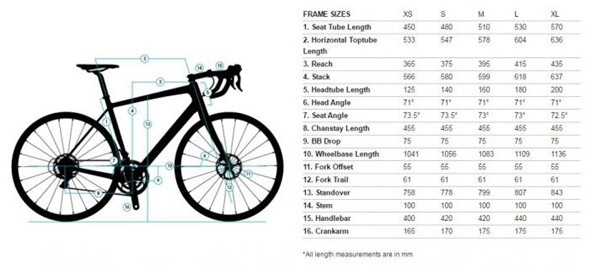
\includegraphics[width=150mm]{Imagen1.jpg} % archivo
    \caption{Partes de una bicicleta.}
    \label{grafica}
\end{figure}
\newpage
\subsubsection{Longitud del tubo de sillín (Seat Tube Lenght)}
Es la distancia desde el centro del eje de pedalier (Bottom Bracket, BB en adelante) hasta el punto más alto del tubo. Esta medida suele definir la talla de la bicicleta, dependiendo del fabricante se suelen expresar en centímetros o en pulgadas. \\
En bicicletas de doble suspensión, también se representa una medida virtual de la longitud del tubo de sillín (Seat Tube, ST en adelante), porque la longitud real no representa la talla debido a las formas que suelen utilizar en los tubos para añadir los puntos de unión de la bieleta. 
\begin{figure} [htp]% figura
    \centering
    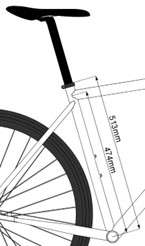
\includegraphics[width=50mm]{Imagen2.jpg} % archivo
    \caption{Longitud del tubo de sillín.}
    \label{grafica}
\end{figure}

\subsubsection{Ángulo de sillín (Seat Tube Angle)}
Es la medida que representa el ángulo formado entre el ST (Seat Tube) y el plano horizontal (Suelo). El rango que los fabricantes solían trabajar estaba entre 69 ° y 74 ° dependiendo de la modalidad. \\
Pero la evolución de la geometría de la bicicleta, la aparición de nuevas modalidades y la implementación de los nuevos tamaños de rueda como de la biomecánica las medidas dieron un gran giro y en concreto el ángulo de sillín (Seat Tube Angle – STA).
\begin{figure} [htp]% figura
    \centering
    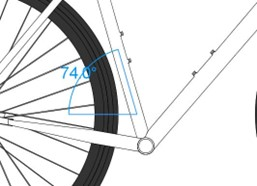
\includegraphics[width=50mm]{Imagen3.jpg} % archivo
    \caption{Ángulo de sillín.}
    \label{grafica}
\end{figure}

\subsubsection{Longitud del tubo de dirección (Head Tube Lenght)}
Esta es una de las medidas que indica las instrucciones ergonómicas del cuadro. \\
La longitud del tubo de dirección (Head Tube Length – HTL) nos va a proporcionar la altura de la parte delantera de la bicicleta haciendo que varíe la posición del ciclista. 
\begin{figure} [htp]% figura
    \centering
    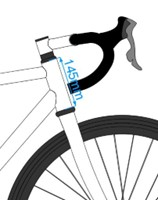
\includegraphics[width=50mm]{Imagen4.jpg} % archivo
    \caption{Longitud del tubo de dirección.}
    \label{grafica}
\end{figure}

\subsubsection{Ángulo del tubo de dirección (Head Tube Angle)}
Es el ángulo que forma el tubo de dirección (Head Tube) con respecto al plano horizontal (Suelo). Influyen directamente en el comportamiento de la bicicleta. Un ángulo de dirección muy abierto ayudará a mejorar las subidas y estable en los tramos llanos, con una posición y manejabilidad más cómoda. También provoca que la bicicleta tenga un comportamiento direccional más directo, nervioso e inestable en las bajadas. Un ángulo de dirección cerrado se emplea en bicicletas de enduro y descenso donde necesitamos que la bicicleta sea estable y ataque muy bien los obstáculos. 
\begin{figure} [htp]% figura
    \centering
    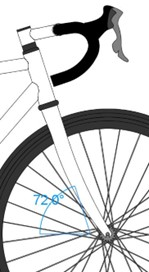
\includegraphics[width=40mm]{Imagen5.jpg} % archivo
    \caption{Ángulo del tubo de dirección.}
    \label{grafica}
\end{figure}
\newpage
\subsubsection{Tubo superior (Top Tube)}
Es el tubo que une el Head Tube (Tubo de dirección) y el Seat Tube (Tubo de sillín). Su medida determina la distancia que hay desde el centro de HT a centro de ST. Su valor varía con respecto a la talla de la bicicleta, siendo mas largo cuando mas grande sea esta.
\begin{figure} [htp]% figura
    \centering
    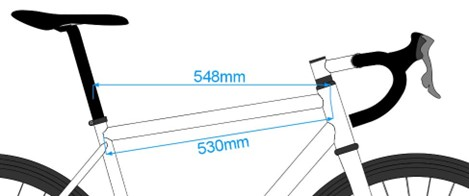
\includegraphics[width=50mm]{Imagen6.jpg} % archivo
    \caption{Tubo superior.}
    \label{grafica}
\end{figure}
\subsubsection{Altura de pedalier (Bottom Bracket Height)}
Es la distancia vertical desde el centro del eje pedalier al suelo. Determinar el espacio que tendrá la bicicleta para superar obstáculos sin golpear con el cuadro o los platos. Espacio determinante para la estabilidad y maniobrabilidad de la bicicleta.
\begin{figure} [htp]% figura
    \centering
    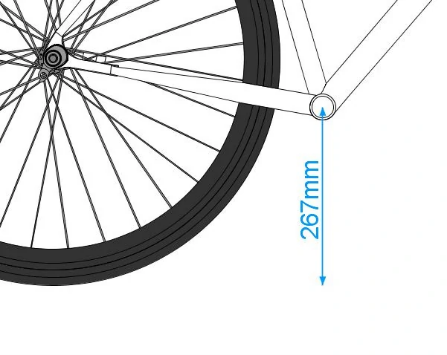
\includegraphics[width=50mm]{Imagen7.png} % archivo
    \caption{Altura de pedalier.}
    \label{grafica}
\end{figure}
\subsubsection{Caída del pedalier (Bottom Bracket Drop)}
Puede parecer que es una medida que va relacionada con la altura de la caja de pedalier, pero no, es totalmente independiente. Distancia que se toma entre la línea horizontal imaginaria que une los ejes de las ruedas y el punto central del eje de pedalier. El valor vertical que hay entre estos dos puntos es el BB Drop (Caída del pedalier).
\begin{figure} [htp]% figura
    \centering
    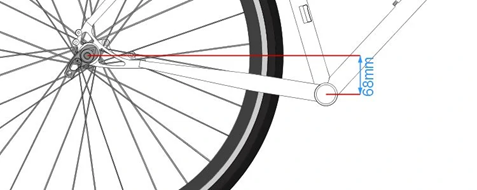
\includegraphics[width=50mm]{Imagen8.png} % archivo
    \caption{Caída del pedalier.}
    \label{grafica}
\end{figure}
\newpage
\subsubsection{Longitud de vainas (Chain Stay Length)}
Es la longitud que existe entre el centro del eje de pedalier y el centro del eje de la rueda trasera. Longitud que hará que la bicicleta sea más o menos estable al mismo tiempo que rápida o lenta en subidas y bajadas.
\begin{figure} [htp]% figura
    \centering
    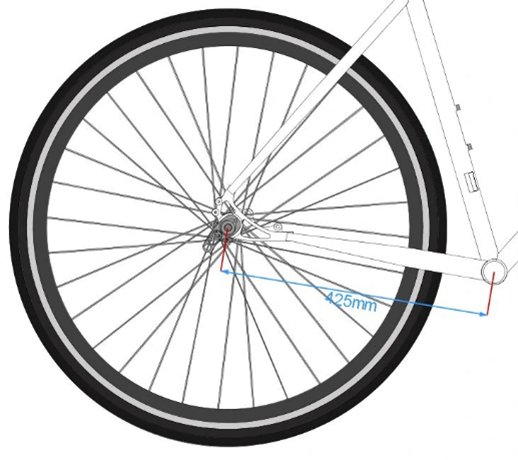
\includegraphics[width=50mm]{Imagen9.png} % archivo
    \caption{Longitud de vainas.}
    \label{grafica}
\end{figure}

\subsubsection{Reach}
Imaginemos una línea vertical que cruza el centro del eje de pedalier. El Reach es la distancia horizontal desde esta línea hasta la parte superior del centro del tubo de dirección.
\begin{figure} [htp]% figura
    \centering
    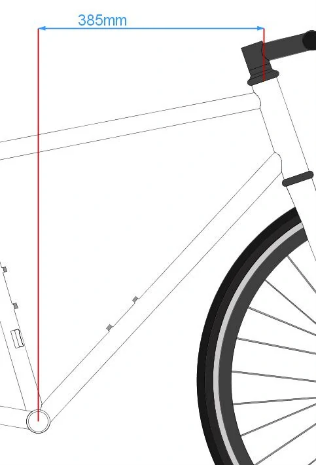
\includegraphics[width=50mm]{Imagen10.png} % archivo
    \caption{Reach.}
    \label{grafica}
\end{figure}

\subsubsection{Stack}
El Stack, o altura del cuadro, es la distancia vertical que existe entre el centro del eje de pedalier y la parte superior del centro del tubo de dirección.
\subsubsection{Offset}
Esta es una de las medidas que más confusión produce en la geometría de la bicicleta junto con el trail. El offset se mide trazando una línea vertical en el eje de la rueda delantera y otra prolongando la línea imaginaria de tubo de dirección. La diferencia de distancia entre una y otra es el Ofsset.
\subsubsection{Trail}
A simple vista podría parecer la misma medida, pero no se parecen en nada. El trail de una horquilla es la distancia entre el punto de contacto de la cubierta con el suelo y donde la línea imaginaria del Head Tube hace contacto con el suelo.
\subsubsection{Distancia entre ejes (Wheel Base)}
En el mundo de la automoción esta medida se conoce como batalla. Cuando hablamos de la geometría de la bicicleta es la distancia que existe entre el centro de los ejes de las ruedas. El Wheel Base varía mucho el comportamiento de la bicicleta tanto en estabilidad como en capacidad de reacción. A menor distancia entre ejes, más rápida de reacción y ágil es la bicicleta, pero a la vez reduce su estabilidad y, sobre todo, la seguridad a altas velocidades. Cuando aumentamos la distancia, la bicicleta es más lenta o torpe en los giros rápidos, pero será mucho más estable y segura a velocidades elevadas.
\subsubsection{Rake}
El rake de una horquilla es el avance del eje de la rueda sobre la línea del tubo de dirección. Dirás que es lo mismo que el Offset, pero no, no es lo mismo. Similar y relacionado.

\subsection{Estado del arte}
La geometría de la bicicleta es algo así como el ADN de la misma. Un error de medidas y el mejor de los modelos puede fallar estrepitosamente. Te explicamos qué son las medidas de una bici y como influyen en su rendimiento.\\
La geometría de una bici mide las longitudes de los tubos que la conforman, así como los ángulos que forman dichos tubos en la dirección y en el tubo de sillín principalmente. Los tubos se miden desde centro a centro y evidentemente no es necesario que la forma de los tubos sea convencional para medirlos. Lo que se mide es la longitud; no importa si el cuadro está realizado en algún tipo de monocasco o con tubería convencional o hidroformada. De este modo, además de la talla, que es el primer parámetro por el que elegimos una bici a nivel de medidas, la geometría es básica para que la bici se comporte de una manera u otra dependiendo del conjunto de medidas y ángulos.\\
\newpage
\subsubsection{Longitudes y ángulos de la MTB}
La geometría de una bici mide las longitudes de los tubos que la conforman, así como los ángulos que forman dichos tubos en la dirección y en el tubo de sillín principalmente. Los tubos se miden desde centro a centro y evidentemente no es necesario que la forma de los tubos sea convencional para medirlos. Lo que se mide es la longitud; no importa si el cuadro está realizado en algún tipo de monocasco o con tubería convencional o hidroformada. De este modo, además de la talla, que es el primer parámetro por el que elegimos una bici a nivel de medidas, la geometría es básica para que la bici se comporte de una manera u otra dependiendo del conjunto de medidas y ángulos.\\
Te explicamos todo con detalle más adelante, pero te queremos contar un poco de antemano por qué la geometría afecta tanto al comportamiento de una bici. Los dos parámetros más importantes de una bici son los ángulos de dirección y de sillín. El de dirección va a hacer que la bici sea más estable, o que gire más rápido y que tenga una mayor viveza de reacciones. Esto sumado a una mayor seguridad a la hora de bajar y una absorción de impactos más efectiva, por el propio ángulo que forma la horquilla sobre el terreno por el que pasamos. Ángulos de dirección más verticales (entre 67 y 70 grados) son más propios de modelos de cross country. Ángulos de dirección más cerrados (64-65 grados), son utilizados en los modelos de enduro. Menos de 64 grados son para modelos de descenso y también para algunos modelos de enduro.\\
En cuanto al ángulo de sillín, determina la posición donde nos sentamos a la hora de pedalear, dependiendo de si estamos muy lejos o demasiado encima del eje de pedalier. Esto influye también en el reparto de pesosde la bici así como en la manejabilidad de la misma. Normalmente oscilan entre los 73 y 77 grados. En los últimos 3 años ha habido un avance muy rápido y radical sobre el ángulo de sillín, ya que se ha ido verticalizando más, hasta llegar a cifras de hasta 76 y 78 grados. Esta tendencia es básica para que el pedaleo sea más efectivo al situarnos más encima en la vertical del eje de pedalier. Y esto se aplica tanto a cross country, como trail, enduro, descenso y también las ebikes.
\subsubsection{Algoritmos evolutivos}
Los algoritmos evolutivos son estrategias de optimización y búsqueda de soluciones que toman como inspiración la evolución en distintos sistemas biológicos. La idea fundamental de estos algoritmos es mantener un conjunto de individuos que representan una posible solución del problema. Estos individuos se mezclan y compiten entre sí, siguiendo el principio de selección natural por el cual sólo los mejor adaptados sobreviven al paso del tiempo. Esto redunda en una evolución hacia soluciones cada vez más aptas\cite{rf1}. \\
Los algoritmos evolutivos son una familia de métodos de optimización, y como tal, tratan de hallar una tupla de valores (xi,...,xn) tales que se minimice una determinada función F(xi,...,xn). En un algoritmo evolutivo, tras parametrizar el problema en una serie de variables, (xi,...,xn) se codifican en una población de cromosomas. Sobre esta población se aplican uno o varios operadores genéticos y se fuerza una presión selectiva (los operadores utilizados se aplicarán sobre estos cromosomas, o sobre poblaciones de ellos). Esta forma de funcionamiento les confiere su característica más destacable: un algoritmo evolutivo puede ser implementado de forma independiente del problema, o a lo sumo, con un conocimiento básico de éste, lo cual los hace algoritmos robustos, por ser útil para cualquier problema, pero a la vez débiles, pues no están especializados en ningún problema concreto siendo los operadores genéticos empleados los que en gran parte confieren la especificabilidad al método empleado\cite{rf3}. 
\newpage
\subsection{Pasos del desarrollo de la programación}
A continuación, veremos la codificación de la programación en MATLAB.
\begin{lstlisting}
%%%% A 99 LINE TOPOLOGY OPTIMIZATION CODE BY OLESIGMUND, OCTOBER 1999 %%%
function topp1(nelx,nely,volfrac,penal,rmin)
% INITIALIZE
x(1:nely,1:nelx) = volfrac;
loop = 0;
for ely = 1:nely
for elx = 1:nelx
 if ((elx)^2+(ely-nely)^2) < (0.65*nelx)^2
 passive(ely,elx) = 1;
 else
 passive(ely,elx) = 0;
 end
end
end
x(find(passive))=0.001;
change = 1.;
% START ITERATION
while change > 0.01
loop = loop + 1;
xold = x;
% FE-ANALYSIS
 [U]=FE(nelx,nely,x,penal);
% OBJECTIVE FUNCTION AND SENSITIVITY ANALYSIS
 [KE] = lk;
 c = 0.;
 for ely = 1:nely
 for elx = 1:nelx
 n1 = (nely+1)*(elx-1)+ely;
 n2 = (nely+1)* elx +ely;
 Ue = U([2*n1-1;2*n1; 2*n2-1;2*n2; 2*n2+1; 2*n2+2; 2*n1+1;2*n1+2],1);
 c = c + x(ely,elx)^penal*Ue'*KE*Ue;
 dc(ely,elx) = -penal*x(ely,elx)^(penal-1)*Ue'*KE*Ue;
 end
 end
% FILTERING OF SENSITIVITIES
%[dc] = check(nelx,nely,rmin,x,dc);
% DESIGN UPDATE BY THE OPTIMALITY CRITERIA METHOD
[x] = OC(nelx,nely,x,volfrac,dc,passive);
% PRINT RESULTS
change = max(max(abs(x-xold)));
disp(['It.:' sprintf('%4i',loop) 'Obj.:' sprintf('%10.4f',c) ...
' Vol.: ' sprintf('%6.3f',sum(sum(x))/(nelx*nely)) ...
' ch.: ' sprintf('%6.3f',change )])
% PLOT DENSITIES
colormap(gray); imagesc(-x); axis equal; axis tight; axis off;pause(1e-6);
end
%%%%%%%%%% OPTIMALITY CRITERIA UPDATE %%%%%%%%%
function [xnew]=OC(nelx,nely,x,volfrac,dc,passive)
l1 = 0; l2 = 100000; move = 0.2;
while ((l2-l1)/l2 > 1e-4)
lmid = 0.5*(l2+l1);
xnew(find(passive))=0.001
xnew = max(0.001,max(x-move,min(1.,min(x+move,x.*sqrt(-dc./lmid)))));
if sum(sum(xnew)) - volfrac*nelx*nely > 0;
l1 = lmid;
else
l2 = lmid;
end
end
%%%%%%%%%% MESH-INDEPENDENCY FILTER %%%%%%%%%%%
function [dcn]=check(nelx,nely,rmin,x,dc)
dcn=zeros(nely,nelx);
for i = 1:nelx
for j = 1:nely
sum=0.0;
for k = max(i-round(rmin),1):min(i+round(rmin),nelx)
for l = max(j-round(rmin),1):min(j+round(rmin), nely)
fac = rmin-sqrt((i-k)^2+(j-l)^2);
sum = sum+max(0,fac);
dcn(j,i) = dcn(j,i) + max(0,fac)*x(l,k)*dc(l,k);
end
end
dcn(j,i) = dcn(j,i)/(x(j,i)*sum);
end
end
%%%%%%%%%% FE-ANALYSIS %%%%%%%%%%%%
function [U]=FE(nelx,nely,x,penal)
[KE] = lk;
K = sparse(2*(nelx+1)*(nely+1), 2*(nelx+1)*(nely+1));
F = sparse(2*(nely+1)*(nelx+1),1); U =sparse(2*(nely+1)*(nelx+1),1);
for ely = 1:nely
for elx = 1:nelx
n1 = (nely+1)*(elx-1)+ely;
n2 = (nely+1)* elx +ely;
edof = [2*n1-1; 2*n1; 2*n2-1; 2*n2; 2*n2+1;2*n2+2;2*n1+1; 2*n1+2];
K(edof,edof) = K(edof,edof) + x(ely,elx)^penal*KE;
end
end
% DEFINE LOADSAND SUPPORTS(HALF MBB-BEAM)
F(2,1) = 1;
fixeddofs =2*nelx*(nely+1)+1:2*(nelx+1)*(nely + 1);
alldofs = [1:2*(nely+1)*(nelx+1)];
freedofs = setdiff(alldofs,fixeddofs);
% SOLVING 127
U(freedofs,:) = K(freedofs,freedofs) \F(freedofs,:);
U(fixeddofs,:)= 0;
%%%%%%%%%% ELEMENT STIFFNESS MATRIX %%%%%%%
function [KE]=lk
E = 1.;
nu = 0.3;
k=[ 1/2-nu/6 1/8+nu/8 -1/4-nu/12 -1/8+3*nu/8 ...
-1/4+nu/12 -1/8-nu/8 nu/6 1/8-3*nu/8];
KE = E/(1-nu^2)*[ k(1) k(2) k(3) k(4) k(5) k(6) k(7) k(8)
k(2) k(1) k(8) k(7) k(6) k(5) k(4) k(3)
k(3) k(8) k(1) k(6) k(7) k(4) k(5) k(2)
k(4) k(7) k(6) k(1) k(8) k(3) k(2) k(5)
k(5) k(6) k(7) k(8) k(1) k(2) k(3) k(4)
k(6) k(5) k(4) k(3) k(2) k(1) k(8) k(7)
k(7) k(4) k(5) k(2) k(3) k(8) k(1) k(6)
k(8) k(3) k(2) k(5) k(4) k(7) k(6) k(1)];
\end{lstlisting}
\begin{figure}[htp] % figura
    \centering
    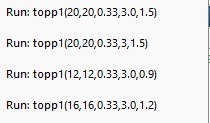
\includegraphics[width=80mm]{Configuraciones.jpeg} % archivo
    \caption{Configuraciones iniciales y análisis de sensibilidad.}
    \label{grafica}
\end{figure}
\newpage
\subsection{Resultados de la optimización}
\begin{figure}[htp]
 \centering
   { 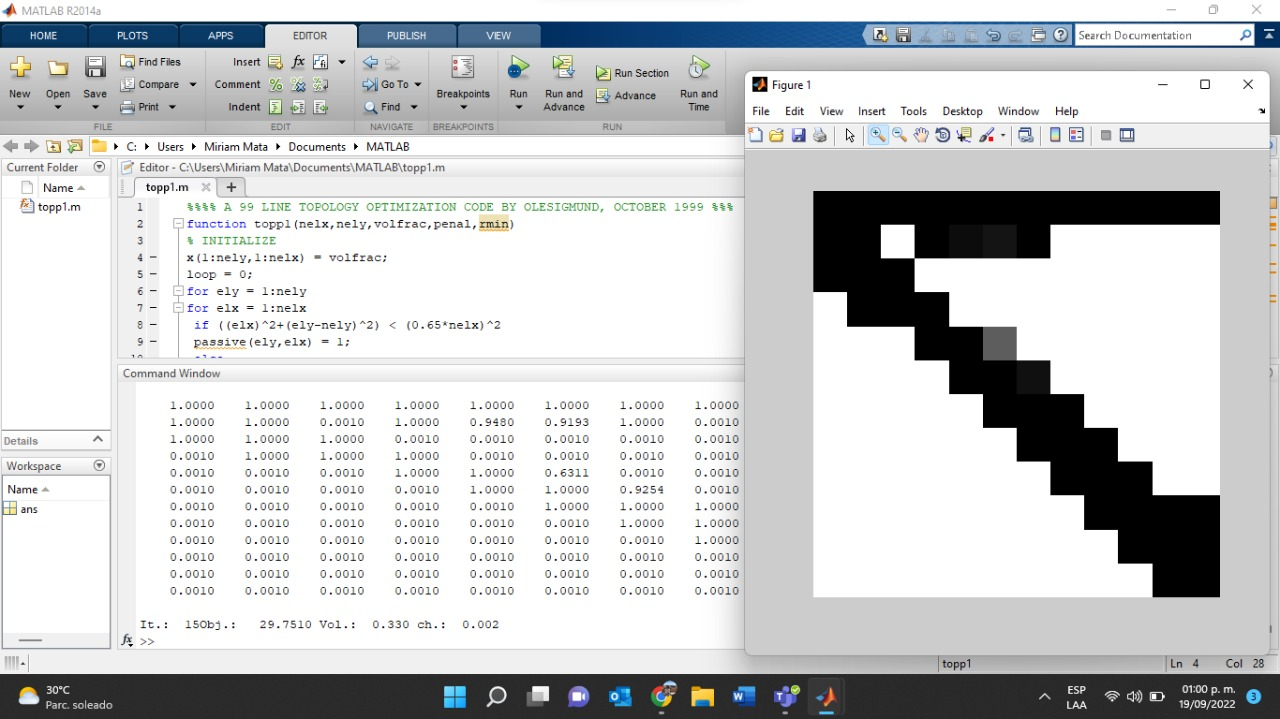
\includegraphics[width=0.85\textwidth]{1.jpeg}}
   {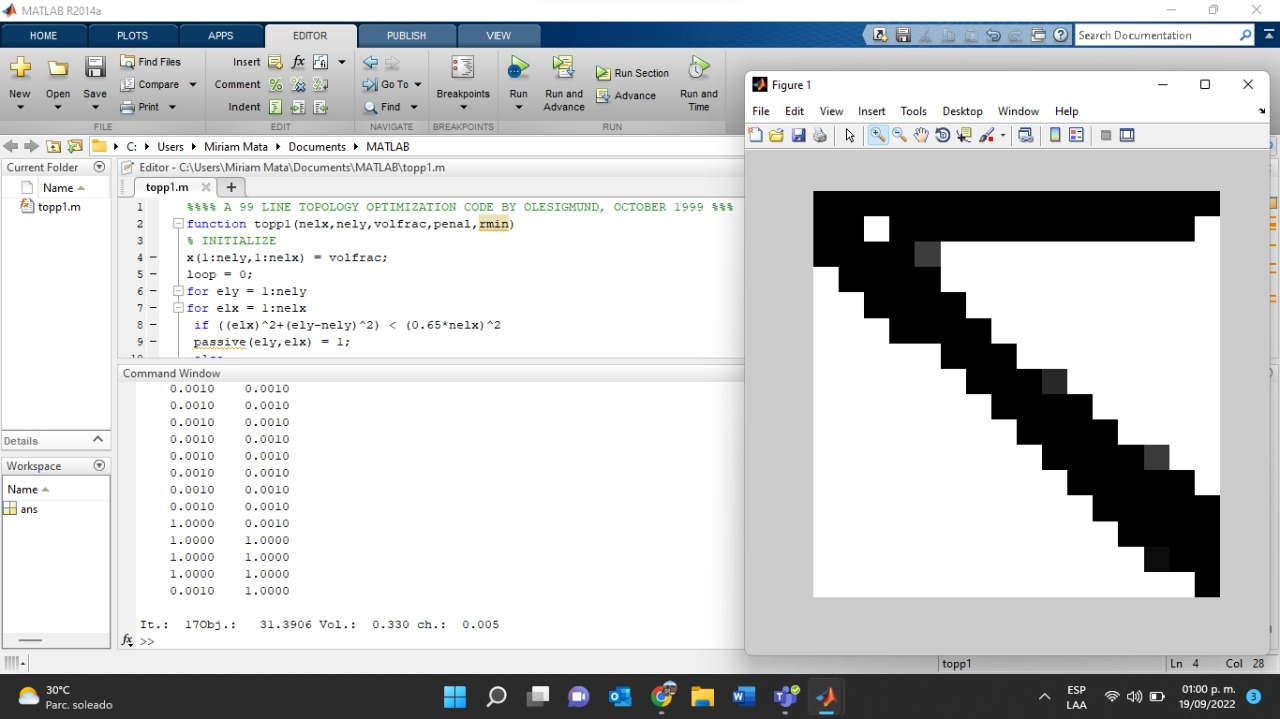
\includegraphics[width=0.85\textwidth]{2.jpeg}}
     \caption{Resultados de la Optimización topológica 1.}
\end{figure}
   
\begin{figure}[htp]
\centering
   { 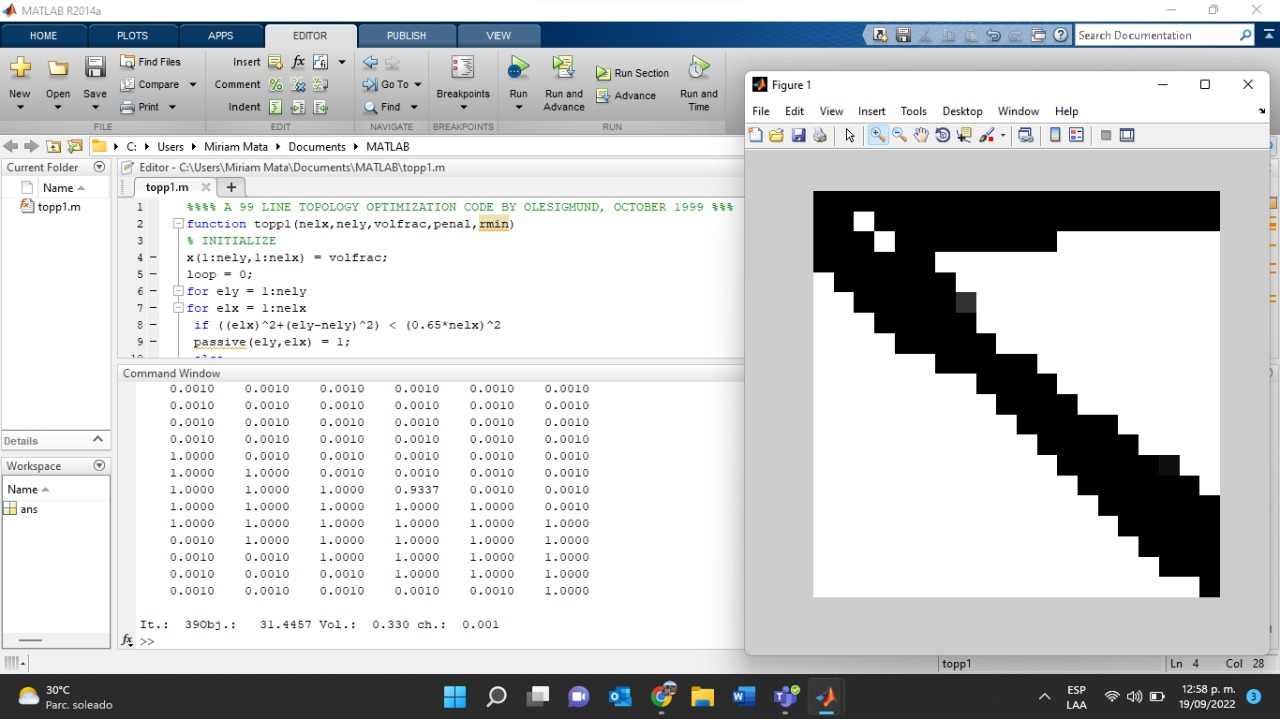
\includegraphics[width=1\textwidth]{3.jpeg}}
    {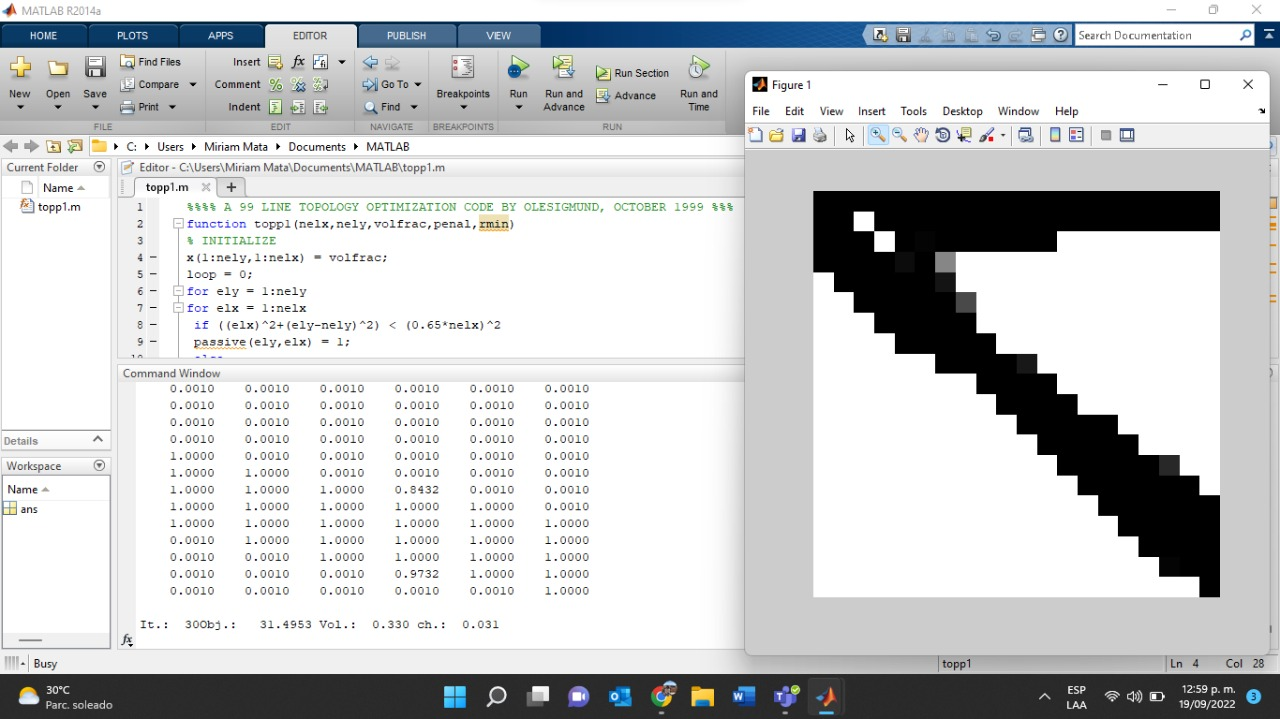
\includegraphics[width=1\textwidth]{4.jpeg}}
  \caption{Resultados de la Optimización topológica 2.}
\end{figure}
   
 \newpage
\section{Conclusiones}
\subsection{Jorge  Fuentes}
Trabajar nuevamente con MATLAB fue gratificante para mí, aplicando lo de la práctica anterior sobre la simulación de matrices llegamos a reforzar los conocimientos comprendidos y volverlos aplicar en esta práctica as entendiendo sobre que estaba haciendo exactamente el código utilizado en nuestra práctica. Una vez entendido fue fácil modificar las variables para ver los resultados que mostraba la optimización de la topología de los elementos que estábamos usando. La ejecución del análisis así como se hace el código en MATLAB fueron de gran ayuda para repasar la programación, ya que, como sabemos la optimización topológica va de la mano con la biomecánica al momento de optimizar los elementos a un grado óptimo y funcional. Me gusto saber mucho sobre la optimización del marco de una bicicleta no sabía mucho sobre sus partes y fue interesante ver estos detalles que desconocía durante la investigación.
\subsection{Tania  Hernandez}
La práctica realizada consistió en la elaboración de un marco de bicicleta o también conocido como cuadro, con el proceso de realización, me pude dar cuenta de lo complejo que es hacerla, desde la parte del funcionamiento que sea practico y aplicable, se puede decir que el marco de la bicicleta, su geometría es realizada con el fin de que la posición y la medida de la persona sea la deseable indicada para el tamaño del cuadro, ya que cada largo, ancho, grados de inclinación, etc., Está pensado para las medidas estándares de cada individuo.
\subsection{Anahi Herrera}
Gracias a la elaboración de esta práctica se entendió de una mejor manera el funcionamiento de MATLAB aplicado hacia la materia de biomecánica, se realizaron investigaciones grupales llevando esta teoría recopilada a la práctica de manera exitosa. 
\subsection{Gustavo  Díaz}
Dentro de esta practica se vio un poco de los temas vistos dentro de la practica pasada por ende se pudieron reforzar dichos conocimientos de la practica pasada al ambas buscar la optimizacion de una pieza esto hace un poco mas sencilla esta practica, en este caso vimos la manera de optimizar la manera de hacer un marco de bicicleta dentro de nuestra investigacion nos dimos cuenta que en como algo tan simple comolo es un marco de bicicleta un cambio de unos milimetros puede hacer que su estructura se vuelva demasiado fragil para poder usarse por ende al hacer la optimizacion fue de ayuda ya que pudimos observar diferenes cuestiones que se ven afectadas al momento de modificarse. Al ser similar a la practica pasada y solo cambiar algunos valores el codigo de la practica pasada nos sirvio de apoyo para esta misma.
\subsection{Miriam  Mata}
Esta práctica estuvo muy interesante porque a pesar de ya haber de usar Matlab en semestres anteriores en lo personal nunca había usado un código como este, fue un poco complicado, pero se logró, siento que a nosotros como futuros ingenieros en mecatrónica se nos debió de haber inculcado más la programación desde los primeros semestres, ya que si bien la mayoría se va a el área de diseño en cierta parte seguimos viendo programación, pero esta actividad me ayudo para poder refrescar un poco mis conocimientos en Matlab porque en sí es un compilador muy sencillo de usar también depende mucho de la librería que te sepas por qué va cambiando cada año.
\subsection{Alejandro Ramos}
En esta práctica me interesó más que ya nos comenzamos a introducir un poco más en el área de ponernos a diseñar algo un poco más avanzado con respecto a lo anterior y que gracias a esto seguimos avanzando en aprender nuevas cosas y el funcionamiento de las herramientas utilizadas me gusta como va desarrollándose las prácticas y espero seguir aprendiendo hasta lograr hacer las cosas lo mejor posible.
\bibliography{bib}
\bibliographystyle{plainnat}
\end{document}
